\documentclass[ASNA,twocolumn]{USG} %twocolumn
\usepackage{anyfontsize} %
\usepackage{colortbl}   % For coloring table lines
\usepackage{xcolor}     % For color definitions

\usepackage{steinmetz}
\graphicspath{{./images/}}

\articletype{ORIGINAL ARTICLE}%
%\subarticletype{xxxx}

%\received{xxxx}
%\revised{xxxx}
%\accepted{xxxx}
\journal{Global Change Biology}
\volume{0}
\copyyear{2026}
\startpage{1}
%\articledoi{10.1002/0000}

\begin{document}
\title{Heatwaves and turbidity influxes have interacting and lasting effects on the foraging behaviour of three-spined sticklebacks \textit{Gasterosteus aculeatus}}
\subtitle{Subtitle}
\transtitle{Functional Response}
\subtranstitle{trans-subtitle}
\author[1]{Cait Newport}[https://orcid.org/0000-0001-6449-7296]
\author[1]{Ellen Morley}
\author[2]{Richard Creswell}
\author[1]{Michelle Jackson}
\author[3]{Ben Lambert}

\authormark{NEWPORT \textsc{et al.}}
\titlemark{Heatwaves and turbidity influxes have interacting and lasting effects on foraging behaviour and freshwater food webs}

\address[1]{\orgdiv{Department of Biology, Oxford, United Kingdom, }\orgname{University of Oxford, }%
\orgaddress{\country{United Kingdom}}}

\address[2]{\orgdiv{Melbourne School of Population and Global Health, }\orgname{The University of Melbourne, }%
\orgaddress{\state{Victoria, }\country{Australia}}}

\address[3]{\orgdiv{Department of Statistics, }\orgname{University of Oxford, }%
\orgaddress{\country{United Kingdom}}}

\corres{Cait Newport  (\email{caitlin.newport@biology.ox.ac.uk})}

\fundingInfo{This research received support through Schmidt Sciences, LLC (to C.N.). \colorbox{yellow}{Add your funding}}

% Include a list of up to six keywords after the abstract
\keywords{Multiple-stressors | fish | acclimation | functional response | food webs}

%\documentclass{USG}  
%\usepackage{amsmath,amsfonts,amssymb}
%\usepackage{graphicx}
%\usepackage{setspace}
%\usepackage{tocloft}
%\usepackage{lineno}
%\usepackage{xcolor}

%Supplementary materials links
%\usepackage[toc,page,titletoc]{appendix}
%\usepackage[hidelinks]{hyperref}
%\newcommand{\suppmat}{\hyperref[sec:suppmat]{Supp.~Mat.}}


%References
%\usepackage[authoryear]{natbib}
\bibliographystyle{wileyNJD-Chicago-lastoo}


%\linenumbers


%\renewcommand{\cftdotsep}{\cftnodots}
%\cftpagenumbersoff{figure}
%%\cftpagenumbersoff{table}
%\begin{document} 
%\maketitle

\abstract[ABSTRACT]{Freshwater ecosystems support a disproportionately high share of fish species and biodiversity, yet are among the most threatened ecosystems globally and are increasingly being exposed to multiple, co-occurring environmental stressors. Yet predicting their combined impacts remains a major challenge, particularly when stressors differ in how quickly they arise and how long their effects persist. Understanding how these stressors interact across time is critical for predicting their ecological consequences. Here, we examine how warming and turbidity—two widespread and intensifying stressors—interact to influence predator–prey dynamics in the three-spined stickleback (\textit{Gasterosteus aculeatus}). Using a fully factorial experiment, fish were exposed to ambient, warmed, turbid, or combined conditions for short (one week) or prolonged (six weeks) periods, before feeding rates were quantified across prey densities using a novel stochastic Bayesian method. We found that foraging behaviour was shaped primarily by prior exposure rather than the immediate experimental conditions. Short-term exposure to both stressors increased feeding performance, whereas prolonged warming reduced feeding efficiency. In contrast, turbidity maintained positive effects over time and, when combined with warming, offset the negative effects of extended heat exposure. Changes in feeding performance at the individual level may propagate through food webs, potentially triggering trophic cascades that reduce biodiversity. Given the exceptional biodiversity of freshwater systems, such dynamics are of particular concern. We also found that behavioural changes persisted even after stressors were removed, indicating that exposure history can have lasting effects. These findings suggest that short-term experiments, such as the functional response, may be actually measuring subject experiential history rather than responses to specific experimental conditions.}

\maketitle

\section{Introduction}\label{sec1}
%\label{sect:intro}  % \label{} allows reference to this section
Freshwater ecosystems support a disproportionate share of global biodiversity \citep{carretevegaWhyAreThere2012} and are among the most threatened environments on Earth \citep{albertScientistsWarningHumanity2021,dudgeonFreshwaterBiodiversityImportance2006}. Their close proximity to human activity combined with limited options for organisms to relocate, can result in organisms being exposed to multiple, often simultaneous, environmental stressors. Among the most pervasive of these stressors are rising temperatures and increasing turbidity. Climate warming is intensifying not only average freshwater temperatures \citep{dokulilIncreasingMaximumLake2021,barbarossaThreatsGlobalWarming2021}, but also the frequency and duration of heatwaves \citep{woolwayLakeHeatwavesClimate2021}. Average lake heatwave temperatures are predicted to increase from 3.7°C to 5.4° and the duration of heatwaves is expected to rise from an average of one week to 12 weeks, under a high-greenhouse-gas-emission scenario \citep{woolwayLakeHeatwavesClimate2021}. Simultaneously, concentrations of both organic and inorganic turbidity are increasing. This increase is driven by both direct human activities, including industrial and agricultural runoff leading to eutrophication \citep{schindlerEutrophicationRecoveryExperimental1974}, dam discharges, and dredging \citep{luNumericalStudyRemote2019,yanEffectsSedimentDredging2023}, and by climate change, which is intensifying extreme precipitation, flooding events, and forest fires \citep{bussiModellingFutureImpacts2016, monierClimateChangeImpacts2015}. As rates of both warming and turbidity continue to increase globally, these stressors are increasingly likely to co-occur \citep{luisvalGlobalChangePhysiological2022}; however, they likely differ in how they affect organisms. 

In fish, the physiological effects of warming have been the focus of studies as warming has been shown to elevate metabolic rates and oxygen demand, while simultaneously reducing the oxygen carrying capacity of water \citep{baileyLinksBehaviourMetabolic2022, holtClimateChangeFish2015,littleWhatWarmingWaters2020}. Turbidity on the other hand, can affect physiology but also sensory function, with impacts that are species, turbidity source, and ecologically context dependent. For example, turbidity can damage gills \citep{cummingGillStructuralChange2016}, reduce visual cue reliability through light scattering \citep{niemanVisualDetectionThresholds2018}, and interfere with olfactory cue detection \citep{aurangzebOlfactorySensoryNeurons2025}. As a result, turbidity can alter how fish acquire information about their environment, including cues related to prey capture and mate selection \citep{zanghiImpactIncreasingTurbidity2025}.

Environmental stressors vary not only in intensity but also in the timescales over which they act. In freshwater systems, turbidity can increase rapidly (e.g.\ minutes to hours) whereas warming develops comparatively slower due to the heat capacity of water (hours to days). Both stressors can persist for extended periods under condition such as eutrophication or prolonged heatwaves. These differences in temporal dynamics mean that fish may experience stressors either as short-term pulses or prolonged exposures, with potentially different consequences for behaviour. Importantly, prior exposure to environmental stress may modify subsequent responses, such that changes in behaviour may reflect not only current conditions but also exposure history \citep{butzgeEarlyWarmingStress2021,chenPreviousExperienceAlters2022,martinPreviousOilExposure2020}.

Alterations in individual behaviour are particularly important in trophic interactions, where changes in individual behaviour can scale up to influence population and community dynamics. Food webs are largely understudied in a multiple stressor context, but they are important to understanding how individual responses cascade to influence the other species they interact with, either as predator or prey. One way to quantify such effects is through functional response experiments, which describe how prey consumption varies with prey density and allow estimation of key behavioural parameters such as attack rate and handling time \citep{hollingCharacteristicsSimpleTypes1959,hollingFunctionalResponseInvertebrate1966}. This framework provides a mechanistic link between environmental conditions and predator–prey interactions, making it well suited to assessing how multiple stressors alter foraging  and its potential long-term effects on food webs and ecosystem dynamics.

We used the three-spined stickleback (\textit{Gasterosteus aculeatus}), a visually oriented mesopredator, and a well-established model species in behavioural and ecological research. Sticklebacks are widely distributed across freshwater systems in the Northern Hemisphere \citep{fangWorldwidePhylogenyThreespined2018} and have been extensively used to study foraging, sensory ecology, and responses to anthropogenic stressors \citep[e.g.][]{haniEffectsChronicExposure2019d,huntingfordThreespinedSticklebacksGasterosteus2009, pottingerIndicesStressThreespined2011, pottingerStressResponseThreespined2013}. This species is generally known to have a wide thermal tolerance but the degree of warming predicted under a high-greenhouse-gas-emission scenario for an extended period still causes higher mortality and higher energy requirements \citep{devergneImpactsLongTermExposure2023}. 

Three-spined sticklebacks are also sensitive to turbidity. This species relies heavily on visual cues for a range of behaviour including predation and sexual selection \citep{huntingfordThreespinedSticklebacksGasterosteus2009, ibrahimRoleVisualCues1989} and turbidity has been shown to disrupt these behaviours. For example, turbidity can weaken sexual selection \citep{candolinChangedEnvironmentalConditions2007}, alter courtship displays \citep{engstrom-ostHumaninducedWaterTurbidity2007}, and affect shoaling \citep{macgregorShoalingBehaviourResponse2023}. It also influences foraging. Moderate levels of bentonite clay induced turbidity can reduce reactive distance to prey, but without necessarily decreasing overall consumption \citep{quesenberryInfluenceTurbidityThreespined2007}, and in some cases increasing attack rates \citep{vollsetInterplayIndividualInteractions2011}. The lack of effect on consumption may reflect a shift towards the use of other sensory modalities, such as olfaction, which can become more important when visibility is reduced \citep{websterTurbidityForagingRate2007}. However, algal-induced turbidity has been shown to reduce both prey consumption and prey selectivity in this species \cite{sohelEffectsTurbidityPrey2017}. Therefore, the responses of three-spined stickleback to warming and turbidity are complex and may depend on a range of factors including exposure history, magnitude of the stressor, turbidity type, and the mechanism underlying behavioural change. It remains unclear how these stressors will interact: effects may be additive through shared physiological pathways, or turbidity-induced sensory impairment may be mitigated by the use of alternative sensory systems. 

To disentangle the effects of stressor type and exposure duration, we experimentally tested how warming and turbidity, individually and in combination, affect fish foraging behaviour. In this fully factorial experiment, fish were exposed to ambient, warmed, turbidity, or combined warming and turbidity treatments, for either 1 week, or 6 weeks. Following these exposure periods, we quantified prey consumption using a functional response approach, measuring feeding rates across seven prey densities during a standardized one-hour feeding trial conducted under each of the four environmental conditions. This design allows us to assess whether behavioural responses are driven primarily by immediate environmental conditions or by the duration of prior exposure. 

\section{Methods}

\subsection{Study species}

A total of 672 wild-caught sticklebacks from several freshwater waterways within England were used. Authors CN and EM caught 158 fish from Lincolnshire, UK (November 2021). All remaining fish were purchased from a local supplier (DC Freshwater Fish Ltd.) in Nottingham. Experimental protocols and husbandry were carried out in accordance with the University of Oxford, Department of Biology Local Ethical Review Committee (AWERB: APA\slash 1\slash 5\slash ZOO\slash NASPA\slash Newport\&Jackson\slash Sticklebacks). Fish sex was not identified as the study occurred outside of the UK breeding season so external indicators were not visible. Experiments were undertaken between November 2021 and March 2022. 

\subsection{Acclimation}

During acclimation, fish were held in a flow-through aquarium system. Each tank was 58L (350 x 300 x 600 mm) and fish were maintained at a stocking density of \begin{math}<\end{math}0.3 fish\slash litre (15 - 17 individuals per tank) with a 12:12 hr photoperiod. Water chemistry was regularly measured and maintained at healthy levels (salinity: 0.002-0.004; pH: 7-7.8; Ammonia: 0ppm; Nitrite: 0ppm; Nitrate: \begin{math}>\end{math}10ppm). All tanks had at least one plastic plant to provide shelter. 

Fish were acclimated within the flow-through aquarium system to one of four conditions (Fig. \ref{fig:fig1}): 1) Ambient: 15°C clear water, 2) Warmed: 20°C clear water, 3) Turbid: 15°C turbid water, and 4) Mixed: 20°C turbid water. Turbid water was created by adding 0.47g of bentonite clay per litre, generating a turbidity level of 28.94±0.91 Nephelometric Turbidity Units (NTU). Bentonite clay was selected as a turbidity source as it appears similar in colour and particle size to the turbidity source found at our field site, and it has been used in previous studies with this species \citep{quesenberryInfluenceTurbidityThreespined2007}. During acclimatisation periods, turbidity was checked twice daily and resuspended by manual mixing with a hand. Temperature was controlled using a water chiller for cold water or ambient room temperature for warm water. Temperature was recorded throughout using HOBO loggers (HOBO UA-001-64). For each condition, fish were assigned to either a one- or six-week acclimation period. Fish were fed twice daily \textit{ad libitum} with defrosted bloodworms and brine shrimp (ratio 2:1). 

\begin{figure*}
\centerline{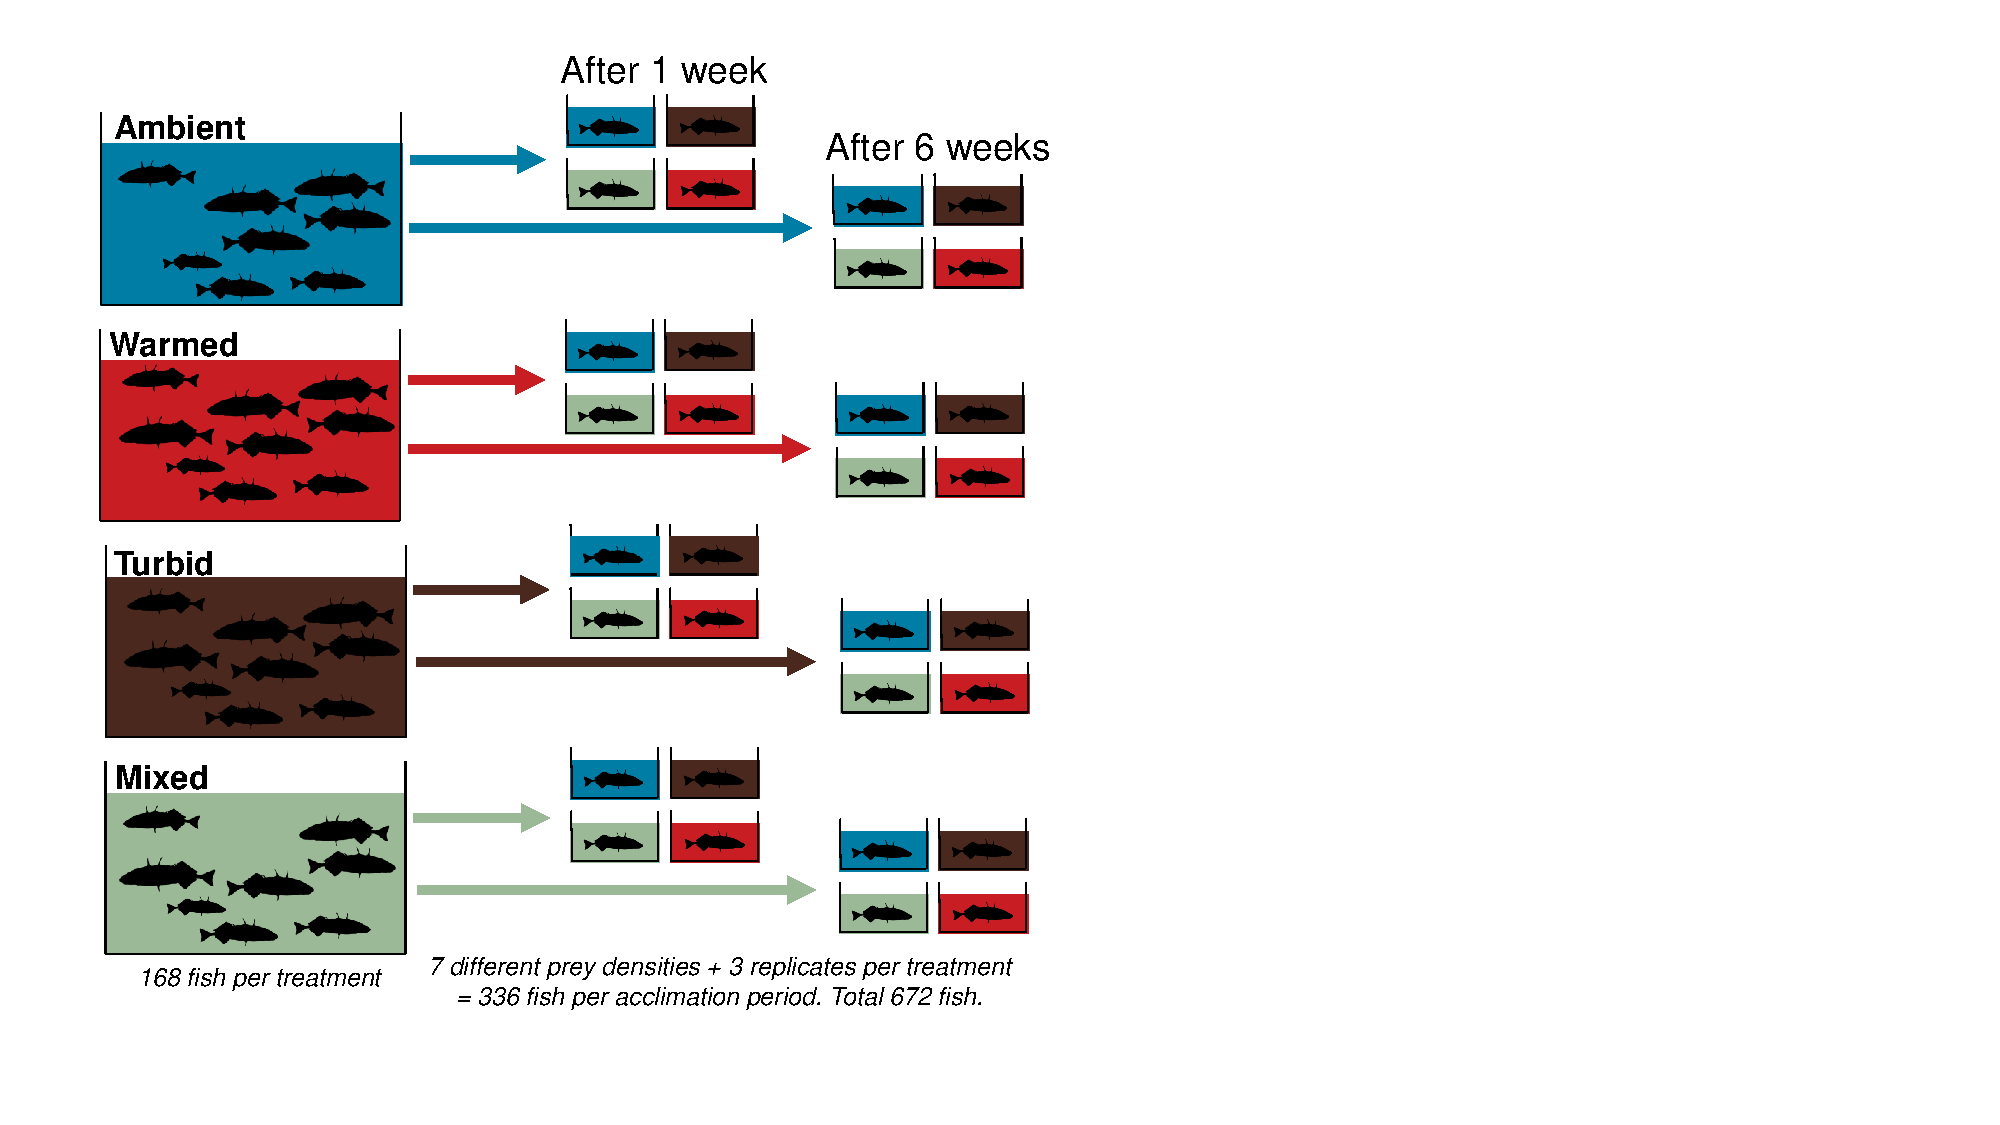
\includegraphics[height=20pc]{figures/Experimental_Design.pdf}}
\caption{Illustration of the fully-factorial experimental sampling procedure.\label{fig1}}
\end{figure*}

\subsection{Functional response (FR) experiment}

Each experimental tank contained one of seven possible prey densities (5, 10, 15, 20, 25, 30, 40 live bloodworms) and one of four water treatments (ambient, warmed, turbid, mixed). The warming treatment was achieved by placing the tank in either a 15°C or 20°C water bath. An extra tank in each water bath contained a submerged logger, measuring temperature at 15-minute intervals, and was used to verify temperature consistency. The experimental turbidity level was 99.28±0.328 NTU (mean ± sd), generated using 1.02 g/L of bentonite clay. Note that the turbidity level was lower during acclimation to ensure fish could be observed during twice daily animal health checks. The experimental turbidity level of ~100 NTU is similar to the level used in previous studies \citep[e.g.][]{abrahamsRoleTurbidityConstraint1997,johannesenOlfactoryCueUse2012} and maximal levels measured in potential \textit{G. aculeatus} habitats in the United Kingdom \citep{ukenvironmentagencyNationalRealTime2015}. To reduce the effect of particle settlement, turbidity was resuspended in all tanks using an electric frother midway through the one-hour experimental period. To ensure all fish experienced the same treatment, even tanks with clear water were mixed. At the end of each experiment, turbidity was remeasured in each turbid tank (mean turbidity = 42.037±1.6NTU). 

Fish were not fed within 24 hours before experiment began. Experiments begun by transferring fish from their acclimation tanks to individual experimental tanks (250x158x128mm). Fish were caught by hand net and placed in a clear bag with 200mL of water from their home tank. The bag was then suspended for 15 minutes within a 3L water bath matching the water temperature that the fish were being moved to. This step was introduced to reduce the risk of stress caused by large temperature changes. After this stage, fish were then transferred directly into their experimental tank by hand net. Fish were given one hour to eat freely and at the end of this period the number of bloodworms remaining in the tank was counted. Three fish replicates were conducted for each treatment condition and prey density. Because of the time required to run experiments, replicates were conducted on consecutive days (28 fish run per day).  After 1 hour, fish were removed from their tank by hand net and transferred directly to a solution of Tricaine mesylate (MS222; 1g MS222 + 3g bicarbonate soda per litre of water) and euthanised and the remaining prey items were counted. Fish total length, standard length and weight were measured. 

We recorded trials using a GoPro Hero5 mounted on a second opaque tank placed directly on top of the tank containing a fish. Only a segment of each trial was filmed due to limitations in camera availability (7 cameras used). Each fish on a given experimental day was randomly assigned to one of four filming groups and each group was filmed for 8 minutes of the experiment (1080 x 1920 pixels; 60 frames per second, fps). These videos were not included in the experimental analysis but the procedure is reported because the presence of recording equipment could influence fish behaviour.  

\subsection{Statistical methods}
\subsubsection{Mechanistic model}
In order to represent the feeding behaviour of fish in our experiments, we developed a novel mechanistic model. This model is inspired by the functional response literature, where the original form of the mathematical models were devised by Holling in 1959, and were justified through simple laboratory-based experiments that timed how long it took human participants to pick up ``discs'' from a table \citep{hollingCharacteristicsSimpleTypes1959}. These mathematical forms, and expanded versions of these, have been used as part of differential equation-based descriptions of predator-prey systems \citep{rosenbaumFittingFunctionalResponses2018a}, which has underpinned popular software used to estimate functional responses from data \citep[e.g.][]{pritchardFrairPackageFitting2017}. Existing approaches, to our knowledge, however, do not explicitly allow for individual-level stochasticity in predation; nor do they strongly justify the somewhat heuristic link between Holling's original toy model and its use as part of a differential equation (albeit some have attempted this in a broader setting of population dynamics models \citep{dawesDerivationHollingsType2013}.

Instead, our approach aims to more directly and explicitly model the searching and consumption of prey. Our model is also stochastic and individual-based to allow for random variation across fish and time in these behaviours. This stochasticity is essential because the number of prey in each treatment of the experiment is relatively few, and only a single fish (the predator) \colorbox{yellow}{is in each replicate}.

We model fish as being in one of two states: \textbf{an active preying (AP)} state and a \textbf{between-preying (BP)} state. The AP state represents periods when fish are actively seeking prey, while the BP state encompasses times when they are not—for instance, due to digestion, doing something unrelated to preying, or a lack of motivation to feed (in the functional response literature, this is typically classed as a prey ``handling'' behaviour but we broaden its definition here to recognise it covers a range of other behaviours). We assume that the duration of the AP state depends on prey density: if there are more prey, it takes less time to find and capture a prey item; and that the duration of the BP state is independent of prey density.

The transitions between the AP and BP states can be described using chemical reaction-like equations: 

\begin{equation}
\label{eqn:eqn1}
1 \text{ AP} +1 \text{ prey} \xrightarrow{a} 1 \text{ BP},
\end{equation}
\begin{equation}
\label{eqn:eqn2}
1 \text{ BP} \xrightarrow{r} 1 \text{ AP},
\end{equation}

where eq.\ (\ref{eqn:eqn1}) represents the capturing of a prey item by a fish in the AP state, which leads the fish to transition to the BP state (e.g.\ when it handles and digests the prey item); the parameter $a>0$ represents the rate at which this capture occurs; eq.\ (\ref{eqn:eqn2}) represents the rate at which the fish in the BP state then reverts to the AP state when it then actively seeks prey; the parameter \begin{math}r > 0\end{math} represents the rate at which this process occurs; \begin{math} h = 1/r\end{math} represents the average time a fish remains in the BP state, and, in the functional response literature, is known as the \textit{prey handling time}.

For brevity, we refer to \begin{math}\alpha\end{math} as the \textit{rate of prey capture} and \begin{math}r\end{math} as the \textit{rate of prey handling}, whilst recognising that biological interpretation of these rates is wider than this terminology.

Eq.\ (\ref{eqn:eqn1}) depends on the availability of a prey item, so the rate at which any prey item is captured is given by \begin{math} N a\end{math}, where \begin{math} N \geq 0\end{math} is the number of prey still available to capture (i.e.\ not already eaten). Eq.\ (\ref{eqn:eqn2}) is \textit{independent} of prey density, so the aggregate rate is just \begin{math}r\end{math} since there is a single predator.

In our experiments, fish are put in enclosures with a given fixed number of initial prey, \begin{math} N_0 > 0\end{math}. This means that, initially, the rate of capture of prey is greatest at \begin{math} a N_0\end{math}, which then decreases linearly as prey are consumed.

\subsubsection{Incorporating covariates}

The fish are exposed to two conditions: the acclimation conditions (i.e. the pre-experimental conditions) and the experimental conditions (i.e. the conditions the fish experience during the hour when the experiment takes place). 

The fish are also heterogeneous; a key source of heterogeneity is their weight, which affects the number of prey fish eaten during an experiment – the heavier the fish, the more it eats \citep{beukemaPredationThreeSpinedStickleback1968}. 

The full set of covariates used in our model included fish weight and its squared term (as model comparison indicated that including this term improved model fit; see Table \ref{tab:model_comparison}), as well as binary variables associated with acclimation and experimental conditions. For each of the acclimation and experimental conditions, four treatment conditions were defined: \textit{ambient}, \textit{warmed}, \textit{turbid} and \textit{mixed}. We additionally included a binary variable which captured the \textit{duration} of time the fish were exposed to the acclimation condition (1 week vs.\ 6 weeks). Interactions between acclimation condition and acclimation duration were also incorporated, as exploratory data visualisations suggested that the magnitude and direction of associations varied with acclimation duration. 

We allowed the rates of prey capture, \begin{math}a\end{math}, and rate of prey handling, \begin{math}r\end{math}, to vary systematically across replicates according to covariates:

\begin{equation}
\label{eqn:eqn3}
\log a = c_a + \beta'_a x_a,
\end{equation}
\begin{equation}
\label{eqn:eqn4}
\log r = c_r + \beta'_r x_r,
\end{equation}

where \begin{math}x_a\end{math} is a vector of covariates associated with variation in the rate of prey capture and \begin{math}x_r\end{math} is a vector of covariates associated with variation in the rate of prey handling. By fitting the model to our experimental data, we estimate \begin{math} c_a, \beta_a, c_r, \beta_r\end{math} , where \begin{math}c_a\end{math} and \begin{math}c_r\end{math} are scalar constants, and \begin{math}\beta_a\end{math} and \begin{math}\beta_r\end{math} are vectors of coefficients of the same length as \begin{math}x_a\end{math} and \begin{math}x_r\end{math}, respectively. 

It was unclear a priori which sets of covariates should be associated with either prey capture (i.e.\ eq.\ \ref{eqn:eqn3}) or prey handling (i.e.\ eq.\ \ref{eqn:eqn4}), so we fitted two models to the data. We chose these two models since we viewed each as equally biologically plausible. These two models included: 
\begin{itemize}
  \item A model where all covariates except those relating to weight were associated with variations in \begin{math}a\end{math} and only the weight variables were associated with variations in \begin{math}r\end{math};
  \item A model where \begin{math}a\end{math} was assumed to be constant (i.e.\ eq.\ \ref{eqn:eqn3} became just \begin{math}\log a = c_a\end{math}) and all covariates were assumed to be associated with variations in \begin{math}r\end{math}.
  \end{itemize}

To choose between these two models, we performed model comparison (described in the \textit{inference} section).

\subsubsection{Inference}
In each of our experimental replicates, we record only the number of prey remaining \textit{at the end} of 1 hour. Each experiment had potentially a range of covariates and differing numbers of initial prey, \begin{math}N_0\end{math}. We fitted our models to all these data simultaneously.


We performed Bayesian inference to infer \begin{math} (c_a, \beta_a, c_r, \beta_r)\end{math} for each of our two models. Bayesian inference requires a prior probability distribution and a likelihood: we chose uninformative independent standard Gaussian (mean $0$, standard deviation $1$) priors on each of our inferred parameters’ values. Specifying the likelihood required determining the probability distribution over the number of prey remaining at the end of a given experimental replicate. In \colorbox{yellow}{\hyperlink{supp:S1}{Supplementary File S1}}, we explain how this probability distribution was derived. There was negligible measurement error in the number of prey remaining at the end of each experimental replicate (this simply involved counting the number of bloodworms still alive). Uncertainty in the final number of prey remaining then stemmed only from variation inherent in the underlying stochastic reaction equation system.  


\begin{table*}[!t]%
\centering %
\caption{Model comparison results. The model in the top row has the point estimate of the best fit to the data. ELPD stands for the expected log-pointwise predictive density and is a measure of model fit (higher values indicate better fit) and Delta ELPD is the difference in ELPD versus the best fitting model; SE Delta(ELPD) represents the standard error of the component-wise difference in ELPD versus the best fitting model. Z represents a z-statistic calculated by dividing the previous two columns, and p indicates a p value versus the null hypothesis that there is no difference in fit versus the best fitting model.\label{tab:model_comparison}}%
\begin{tabular*}{\textwidth}{@{\extracolsep\fill}lcccc@{\extracolsep\fill}}
\toprule
\textbf{Model} & \textbf{Delta ELPD}  & \textbf{SE Delta (ELPD)}  & \textbf{z}  & \textbf{p} \\
\midrule
All h + w + w\begin{math}^{2}\end{math} & -  & -  & -  & -  \\
Mostly a + w + w\begin{math}^{2}\end{math} & -103.11  & 36.20  & -2.85  & \begin{math}<\end{math}0.01   \\
All h + w & -127.96  & 23.59  & -5.43  & \begin{math}<\end{math}0.01   \\
Mostly a + w & -208.19 & 36.80 & -5.56 & \begin{math}<\end{math}0.01  \\
\bottomrule
\end{tabular*}

\end{table*}


To estimate the \textit{posterior distribution} over the model parameters, we used Markov chain Monte Carlo (MCMC) -- specifically, the Haario-Bardenet MCMC algorithm as implemented in PINTS \citep{michaelclerxProbabilisticInferenceNoisy2019}. To initialise the Markov chains, we performed a set of 10 optimisations using the CMAES algorithm as implemented in PINTS and chose the set which had the highest log-posterior score; we chose this approach to initialising the chains as it reduced the time taken for the Markov chains to appear converged versus an alternative approach where chains were initialised by sampling from the prior; this two-step approach potentially risks biasing Markov chains to a particular mode, although we found that often the chains did explore widely during sampling. We performed a total of 50,000 MCMC iterations, and discarded the first 25,000 as burn-in. To assess convergence, we required that the Gelman R-hat statistic \begin{math}\hat{R} < 1.05\end{math} for all model parameters \citep{vehtariPracticalBayesianModel2017}. Tables of parameter estimates with quantiles and $\hat{R}$ are given in \colorbox{yellow}{\hyperlink{supp:S3}{Supplementary File S3}}.

%TODO: Reorder Supplementary files. Possibly put S3 into Appendix.


To check the fit of our model to the data, we performed visual \textit{posterior predictive checks}, where we compared the distribution over number of prey remaining (at the end of each experimental replicate) to the modelled equivalent. To perform model comparison, we used an approximate leave-one-out-cross-validation approach as implemented in the loo R package \citep{vehtariPracticalBayesianModel2017}. Allowing for systematic variations in handling time across fish provided a best fit to the data (see Table \ref{tab:model_comparison} for model comparison results). 

Through discussion of our results, we assessed differences between models using a Region of Practical Equivalence (ROPE), which defines a range of values considered too small to be meaningful in practice. Specifically, we examined the posterior distribution of the difference between model estimates and calculated the proportion falling within $\pm 1$ minute (for discussions where handling time was the output), our chosen ROPE based on the scale of the analysis. Differences within this interval are interpreted as practically equivalent, while differences outside it indicate a meaningful advantage of one model over the other. This approach allows us to distinguish statistically detectable differences from those that are large enough to matter in practice. We used a 0.95 probability threshold, such that if at least 95\% of the posterior mass falls within the ROPE we conclude practical equivalence, whereas if at least 95\% falls outside the ROPE on one side we conclude a meaningful difference.

\section{Results}

Experimental trials were completed for a total of 669 individual fish. Our experimental design produced 224 unique treatment conditions with three fish replicates each. However, for six treatments only two replicates were completed, and for two treatments four replicates were completed. These discrepancies were due to experimenter error. The complete dataset used for analysis is included in \colorbox{yellow}{\hyperlink{supp:S2}{Supplementary File S2}}.

\subsection{Statistical model selection}
- We compared four different models (see Table 1) and found that the best-fitting model is 'Mostly a+w'. The visualisations for the chosen model (Fig \ref{fig:fig2}) indicates a reasonable correspondence between the true and simulated data. What this means is that handling time matters most, and implies that the searching time really doesn't vary across treatments. It is probably because this period is so short within the confounds of the small bucket, to really matter.

We also find that size really matters to how many prey a fish eats within the time period. This is pretty intuitive, but it is good that our model shows that we fit the data well across all three fish size categories. 

\begin{figure*}
\centerline{\includegraphics[height=30pc]{figures/can}}
\caption{\textbf{TO BE UPDATED:} Comparison of actual versus simulated data from the mechanistic model.\label{fig:fig2}}
\end{figure*}

\subsection{The effect of experimental treatment on feeding}

Controlling for the acclimation condition, we found minimal association between the type of experimental condition and the estimated handling time (Fig.~\ref{fig:fig3}A).

\begin{figure*}
\centerline{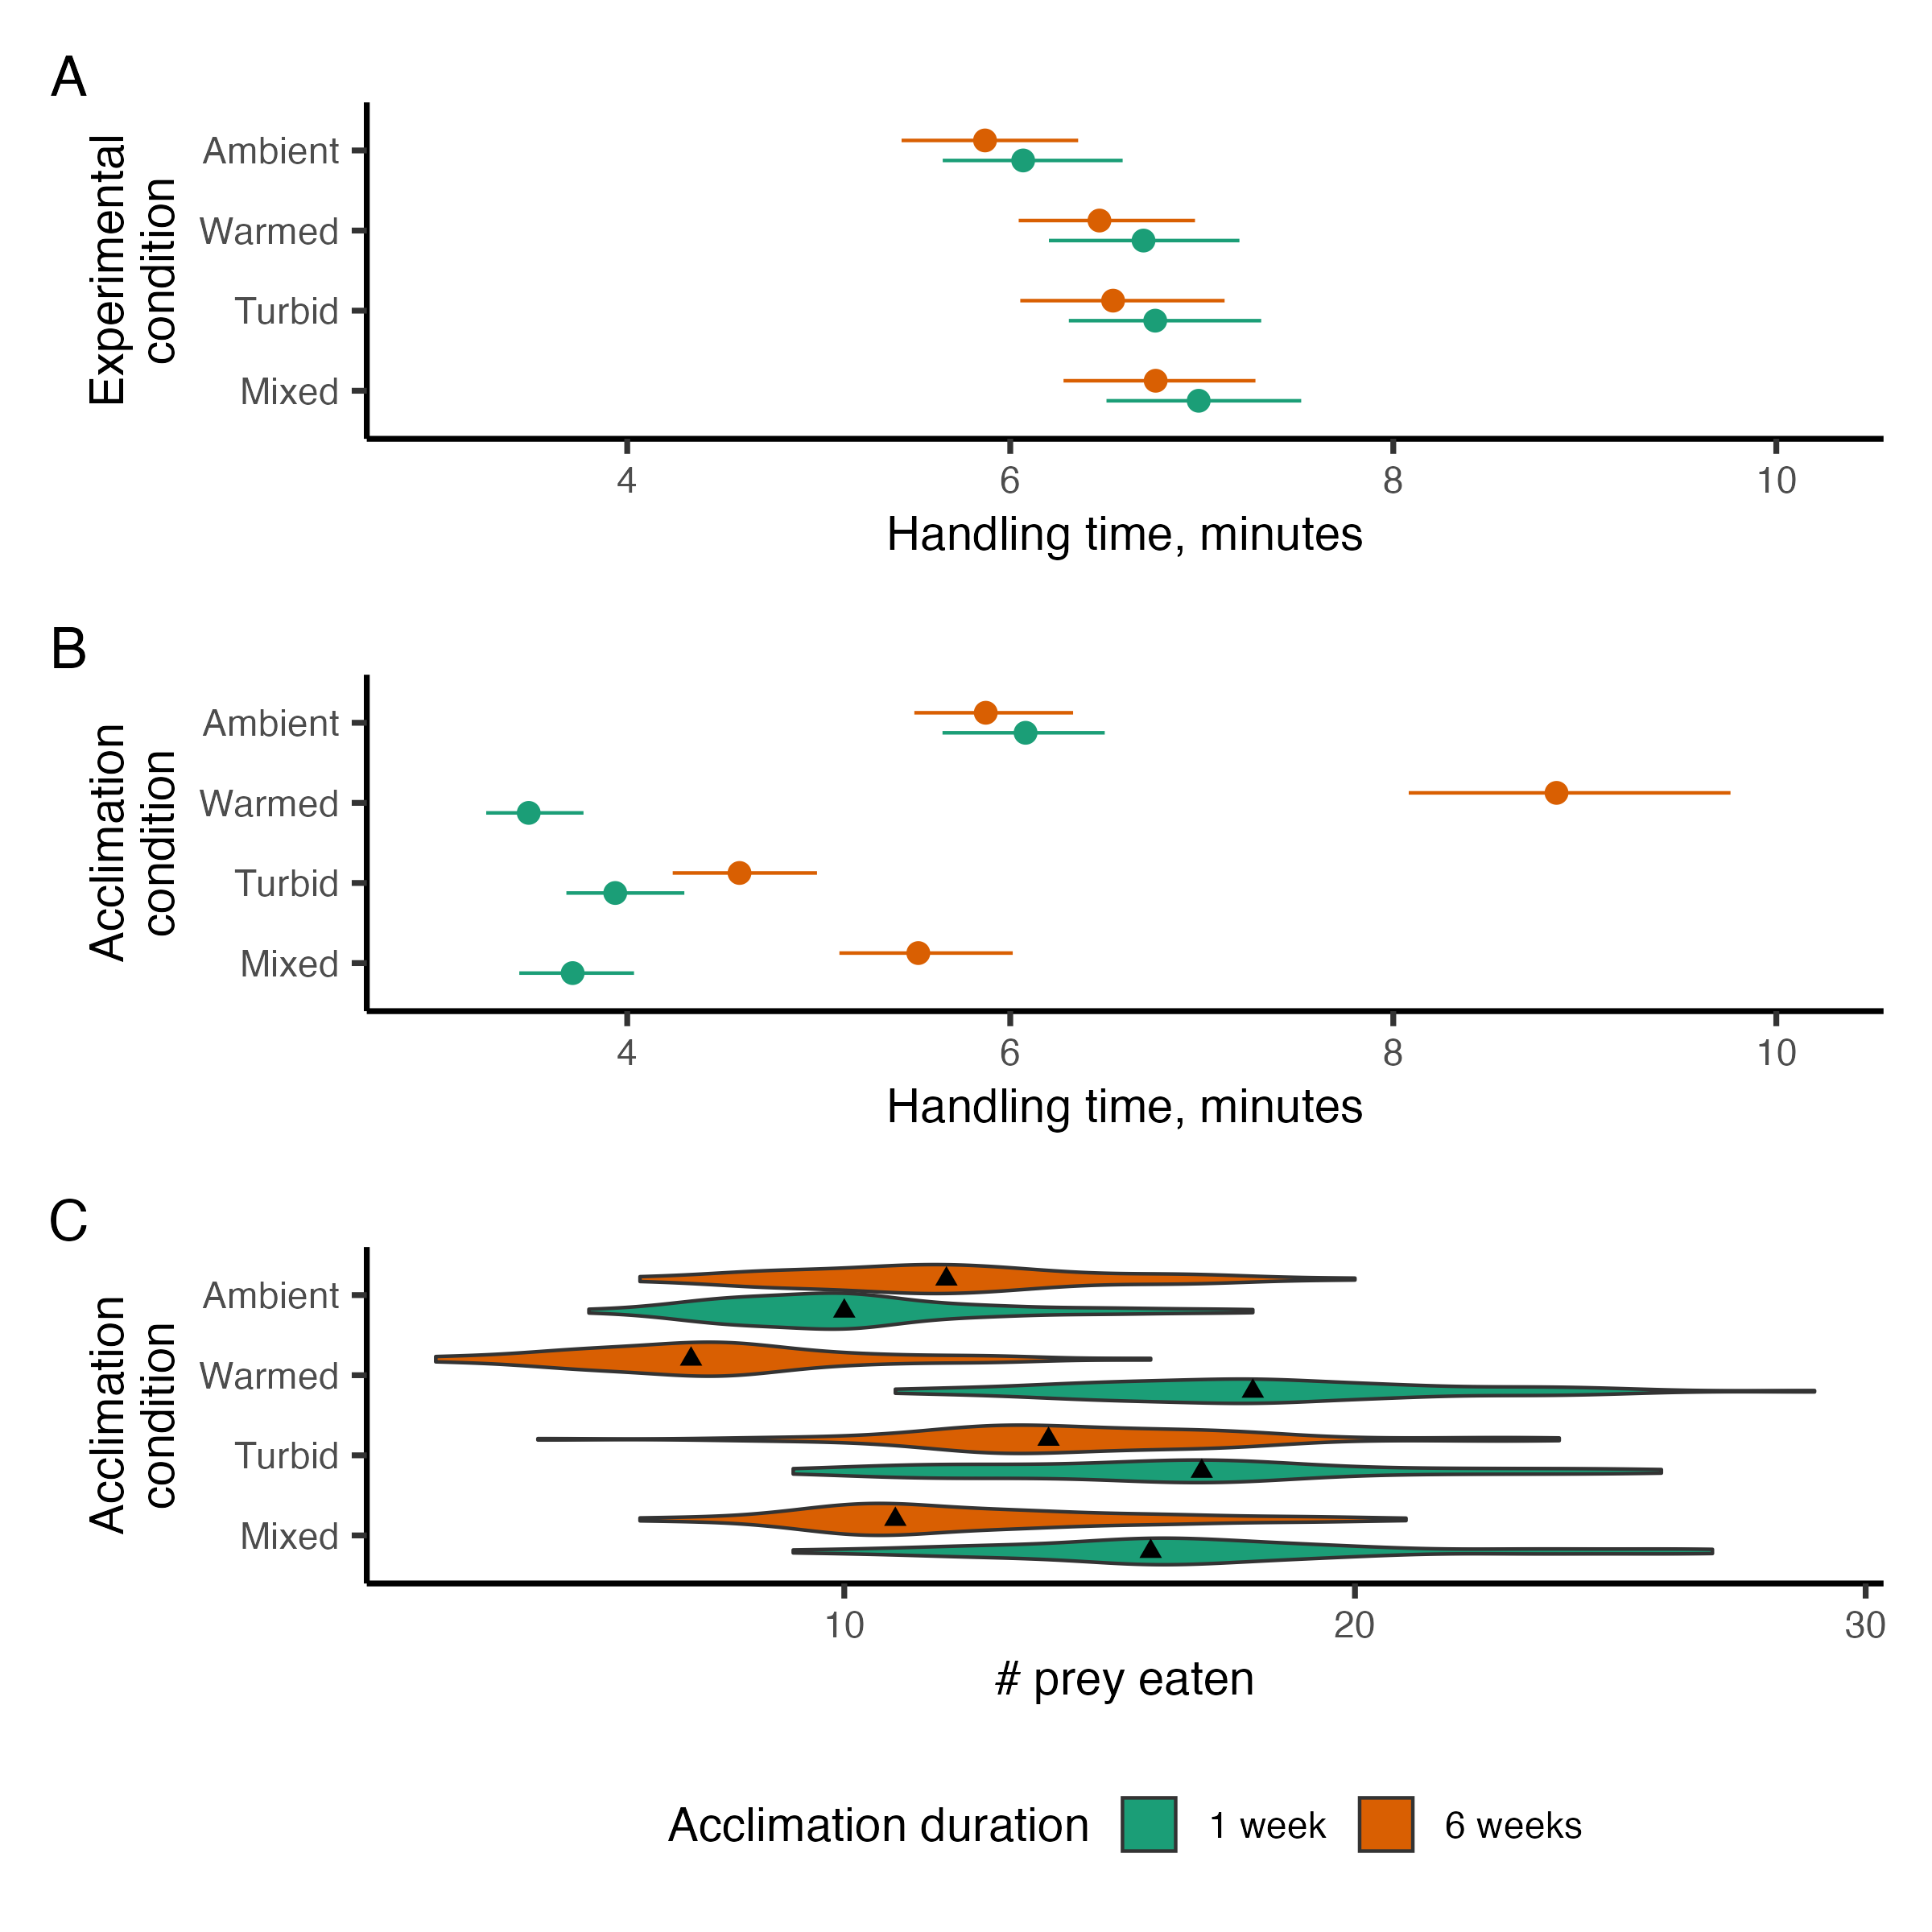
\includegraphics[height=40pc]{figures/combined_three_panel.png}}
\caption{Association between experimental and acclimation conditions and the feeding behaviour of fish. (A) The relationship between the estimated handling time and experimental conditions for fish acclimatised in ambient conditions. (B) The relationship between handling time and acclimation conditions where the experiment was conducted in ambient conditions. (C) The model-predicted number of prey items eaten over the course of a one-hour experiment, where the initial number of prey was assumed to be 40. In all panels, the results are stratified according to the duration of the acclimation period, and the results are generated for a fish of median weight. In A and B, the whiskers show the central 95\% posterior intervals for the handling time; the points show the posterior medians for this quantity. In C, triangles show the posterior medians, and the violins provide kernel density estimates of the distributions.\label{fig:fig3}}
\end{figure*}


\subsection{The effect of acclimation treatment and acclimation duration on feeding behaviour}

There were substantial differences in the estimated handling time across acclimation treatments and durations (Fig.~\ref{fig:fig3}B), with the most pronounced effect under the warmed acclimation treatment. Fish of median weight in the control treatment, maintained under ambient conditions, showed similar handling times regardless of acclimation duration (1 wk:  6.1 min; 6 wks: 5.9 min), and consumed comparable numbers of prey (1 wk: 10 prey; 6 wks: 12 prey) (Fig. 3C). In contrast, fish acclimated to warmed water exhibited a strong duration-dependent response: individuals exposed for one week had a handling time of 3.5 minutes (95\% central posterior interval (95\% CI): 3.3-3.8), whereas those acclimated for six weeks had a substantially longer handling time of 8.9 minutes (95\% CI: 8.1-9.8). Furthermore, our results indicate that fish exposed to warming over longer periods consume considerably more prey than those exposed for shorter periods, and that feeding behaviour differs significantly between both warming treatments and ambient conditions (Fig.~\ref{fig:fig3}C).

% TODO: Check all results values after model is re-run.

Fish acclimated to turbid water also showed marked reductions in handling time compared to those in ambient conditions. However, the magnitude of this effect depended on exposure duration: individuals acclimated for one week had shorter handling times and consumed more prey than those acclimated for six weeks (1 wk: 3.9 min, 17 prey; 6 wks: 4.7 min, 14 prey). Consequently, a 1-week acclimation to turbid water reduced handling time by approximately 35\% for fish of median weight relative to ambient conditions, whereas the reduction after 6 weeks was approximately 22\% (Fig.~\ref{fig:fig2}B).

The effect of combined warming and turbidity (mixed acclimation treatment) was similarly dependent on exposure duration. Fish acclimated under these conditions had shorter handling times than those in ambient conditions, although the magnitude of this effect differed with acclimation length. Fish acclimation for one week exhibited a ~39\% reduction in handling time (3.6 min), compared to only around 6\% (5.7 min) for those exposed for six weeks (Fig.~\ref{fig:fig2}B). Fish in the mixed treatment also consumed more prey than those in ambient conditions. Individuals in the one-week treatment consumed more prey (17 prey) than those exposed for six weeks (12 prey) and both ambient treatments (Fig.~\ref{fig:fig2}C). While handling times were broadly similar across different stressor treatments (warming, turbid, and mixed) after short-term exposure, clear differences emerged following six weeks of acclimation, indicating that longer-term exposure alters the relative effects of these stressors on feeding behaviour.

\section{Discussion}

In this study, we show that the effects of environmental stressors on fish behaviour depend critically on prior exposure conditions. We found that the best predictors for feeding behaviour during the experimental period was not the experimental condition itself, but the acclimation duration and condition the fish were previously exposed to. Across treatments, we found that short-term exposure to warming, turbidity, and their combination, generally increased feeding performance relative to ambient conditions, as indicated by reduced handling times and increased prey consumption. However, these positive effects shifted markedly with prolonged exposure. After six weeks, warming had significant negative effects on feeding performance, whereas turbidity produced positive effects on feeding performance, albeit to a lesser extent than after short-term exposure. In contrast, the mixed treatment led to intermediate outcomes that matched the feeding performance of fish acclimated in ambient conditions, suggesting that the influences of turbidity and warming partially offset one another. Based on these results, conditions most similar to longer duration heatwaves will cause the most significant ecosystem changes. While short heatwaves may initially increase feeding rates and productivity, longer heatwaves will suppress feeding and lead to a subsequent decline in energy intake. As climate change is expected to increase the duration of heatwaves, such shifts from initial 'boom' to subsequent 'bust' phases may have important consequences for predator–prey interactions and the stability of aquatic food webs. 

Sticklebacks occupy a wide range of habitats, including marine, brackish, and freshwater systems, and play an important role in shaping ecosystem dynamics \citep{olinIncreasesOpportunisticSpecies2022}. A growing body of research suggests that, under environmental stress, sticklebacks can increase rapidly in abundance and dominate ecosystems \citep[e.g.][]{bretzelFeedingEcologyInvasive2021,jakobsentsImpactThreespinedStickleback2003}. This success is primarily driven by their broad thermal tolerance, rapid reproduction, and generalist feeding strategy \citep{olinIncreasesOpportunisticSpecies2022}. While such resilience may appear beneficial at the species level, it can have substantial ecological consequences. Sticklebacks are mesopredators, and exert top-down control on prey and high densities of stickleback can reduce the abundance of herbivorous zooplankton and fish eggs \citep{jakobsentsImpactThreespinedStickleback2003, erikssonDeclinesPredatoryFish2009, siebenCascadingEffectsPredator2011, siebenMesopredatorReleaseStickleback2011, candolinEnvironmentalDisturbanceAlters2018}. This can alter food web structure through multiple pathways: egg predation can reduce recruitment of other fish species \citep{kotterbaPredationThreespineStickleback2014, bystromDecliningCoastalPiscivore2015, nilssonPredatorPreyRole2019, donadiPerchPikeRecruitment2020}, while predation on zooplankton can reduce the availability of prey for other predator species leading to resource competition and reduced recruitment success \citep{ljunggrenRecruitmentFailureCoastal2010, bretzelFeedingEcologyInvasive2021}. 

Across all treatments, we observed a Type II functional response, characterised by an increase in feeding rate at low prey densities, followed by a plateau associated with handling time. This type of response implies that predators maintain high consumption rates even at low prey densities, and suggest that there is an increased risk of prey over-exploitation when prey densities are low \citep{hollingCharacteristicsSimpleTypes1959}. Therefore, our results indicate that stressors which decrease handling time and increase predation rate (i.e. 1wk turbidity/warming/mixed and 6wk turbidity) may lead to significant changes in food web structures by reducing the abundance of prey. There is already evidence that such trophic effects can scale up to influence broader ecosystem structure in the Baltic Sea \citep{donadiCrossscaleTrophicCascade2017}. Conversly, our extended heatwave (6wk warming) scenario may lead to reduced predation rates by sticklebacks and thus more abundant and diverse zooplankton communities \citep{jakobsentsImpactThreespinedStickleback2003}. Having more diverse prey could also lead to more larger predators in the ecosystem, so long as those predators do not rely on sticklebacks as their main source of food. However, the reduction in stickleback feeding rate is likely a symptom of decreasing health and fitness. For example, previous studies have shown that sticklebacks kept in warmed water show decreased parental care and reproductive success \citep{hopkinsIncreasedAmbientTemperature2011, haniEffectsChronicExposure2019d}, increased disease susceptibility \citep{karvonenWaterTemperatureNot2013, schadeImpactThermalStress2014, dittmarHeatImmunityExperimental2014}, and decreased growth rates \citep{lefebureTemperaturedependentGrowthModel2011}. If a species known for its broad thermal tolerance changes its behaviour so drastically under heatwave simulated conditions, it is likely that other species in the same ecosystem will fare similarly or worse as water temperatures approach or exceed their thermal tolerance. Therefore, we believe that the decreased handling time and predation rate associated with the 6wk warmed treatment observed in our study, is a strong indicator that these conditions will have significant negative impacts on aquatic ecosystems. 

Increased predation of zooplankton by sticklebacks can have further significant significant ecosystem effects. The zooplankton eaten are often key algal grazers and their depletion can lead to increased algal growth and eutrophication, ultimately increasing turbidity \citep{siebenCascadingEffectsPredator2011, jakobsentsImpactThreespinedStickleback2003, desrochesEcologicalEvolutionaryEffects2013, candolinInfluenceSticklebackAccumulation2016}. Consequently, the increased prey consumption under turbid conditions observed in our study may contribute to a positive feedback loop, whereby sticklebacks further increase turbidity and eutrophication. This effect may be worsened as stickleback populations grow, given that turbidity has also been shown to increase fecundity in this species \citep{saarinenMechanismsBottomupEffects2020}. As not all species benefit from turbidity \citep{rodriguesMetaanalyticalReviewTurbidity2023}, this mechanism may contribute to declines in biodiversity observed in some freshwater systems as stickleback populations expand and displace other species \citep{bretzelFeedingEcologyInvasive2021}. 

Crucially, our results reveal that when stressors co-occur, their effects are not simply additive. Rather than amplifying effects in either direction, the combined influence of warming and turbidity in our experiments appear to counteract one another and potentially offsetting any negative effects \citep{jacksonNetEffectsMultiple2016,piggottReconceptualizingSynergismAntagonism2015}. Therefore, these conditions may result in more stable feeding dynamics. As human induced environmental change is expected to increase both the duration and intensity of heatwaves and turbidity, this finding challenges the assumption that multiple stressors will necessarily intensify ecosystems degradation. Instead, it raises the possibility that, under certain conditions, their interaction could moderate stickleback-driven changes in food webs and even confer a degree of resilience, particularly for species that respond positively to turbidity. 

In this study, we do not directly test the mechanisms underlying changes in feeding behaviour associated with environmental stressors, but we can speculate. The reduction in handling time observed after one week of warming is likely driven by increases in metabolic rate. Previous studies have shown that higher temperatures can accelerate metabolic rate in sticklebacks, resulting in greater feeding and growth rates \citep{guderleyInteractionAgeThermal1994}. But fish have an upper thermal limit beyond which metabolic performance declines \citep{lefebureTemperaturedependentGrowthModel2011}, that may account for the longer handling time observed after prolonged exposure. 

The mechanisms underpinning behavioural responses to turbidity are less well understood. The lack of a behavioural change in fish moved from clear acclimation conditions to turbid experimental conditions (Fig. 2A) suggests that turbidity does not strongly disrupt foraging behaviour in sticklebacks. This contrasts with findings in other species, such as the coral reef triggerfish (\textit{Rhinecanthus aculeatus}), where turbidity has been shown to immediately reduce foraging efficiency, even in the presence of other sensory cues (e.g. olfaction) \citep{newportHighTurbidityLevels2021, rodriguesMetaanalyticalReviewTurbidity2023}. Sticklebacks are known to be visual predators, but from a sensory ecology perspective, our results suggest that turbidity may not limit prey detection, despite it impacting other visually-mediated behaviours such as courtship activity, mate choice, and shoaling \citep{candolinChangedEnvironmentalConditions2007, engstrom-ostHumaninducedWaterTurbidity2007,heuscheleEnvironmentdependentUseMate2009}. Several mechanisms may explain why feeding performance was enhanced under turbid conditions. First, the prey used in our experiments (bloodworms) are relatively conspicuous and presented within a confined space. These conditions may minimize the sensory challenge of prey detection. In addition, we used bentonite clay as a source of turbidity. This material has a slightly red colour and while the increased turbidity will have reduced visual contrast, it may have enhanced or maintained the saliency of the prey colour cue (Garcia et al \textit{in press}). 

An alternative mechanism is that turbidity reduced the visual detection distance of prey, but that this effect was offset through behavioural compensation. Increased turbidity has been shown to reduce predator vigilance in the three-spined stickleback \citep{sohelAlgalTurbidityReduces2015}, allowing individuals to increase prey search effort. To explore the trade-off between decreasing visibility and searching effort, we used simulations. We found search effort, measured as total distance traveled to find all prey, was influenced by both visibility and prey density in our simulations. Under low prey densities, reductions in visibility substantially increased distance traveled: an 88\% decrease in visibility (visual range: 30mm) resulted in a tenfold increase in distance traveled, whereas a 25\% decrease in visibility (visual range: 187.5 mm) led to only a modest (1.06×) increase in distance traveled (Fig. \ref{fig:fig3}). This relationship was non-linear, as the effect size was smaller at higher prey densities. It is important to note that both our experiments and simulations were conducted in confined environments. As such, they do not capture the potential effects of changing visibility in open systems, where an unconstrained random walk could lead to even greater searching distances. The increased activity observed in our simulations suggest that reduced visibility could substantially elevate energetic demands, particularly in low prey density environments. These costs may be further amplified if prey are less conspicuous than the bloodworms used in our experiments, requiring even greater search effort to maintain intake.

A final option is that sticklebacks may adjust sensory sensitivity in response to turbidity over time. For example, they could switch to a potentially more reliable sensory cue in low visibility conditions such as olfaction. However, experiments suggest that olfaction is used primarily to detect the presence of prey rather than locate it, and may instead act to increase the motivation to forage \citep{johannesenOlfactoryCueUse2012}.

Finally, the results of this study highlight an important implication for behavioural research. We found that behavioural change was not driven by the immediate experimental conditions, but instead by the acclimation conditions experienced prior to testing. This suggests that short-term experimental approaches, such as functional response assays, may in effect be capturing prior environmental history rather than responses to the experimental treatment itself. This underscores the importance of accounting for the environmental and experiential history of test subjects when interpreting results \citep{corderyDifferentialCaptivityExperiential2026}. Moreover, the persistence of altered behaviour after fish were removed from their acclimation conditions indicates that prolonged exposure to stressors can have lasting effects, even once conditions return to baseline. In the context of future environmental change, where stressors such as heatwaves and rapid-onset turbidity events are expected to become more frequent, this suggests that behavioural impacts may persist beyond the duration of the disturbance, with recovery occurring over extended timescales. 


%\backmatter
\bmsubsection*{Author Contributions}

\textbf{Cait Newport:} Conceptualization (equal); Investigation (equal); Methodology (equal); Resources (lead); Software (supporting); Supervision (lead); Visualisation (equal); Writing - Original Draft Preparation (lead). \textbf{Ellen Morley:} Investigation (equal); Methodology (equal). \textbf{Richard Creswell:} Software (supporting); Writing - Review \& Editing. \textbf{Michelle Jackson:} Conceptualization (equal); Methodology (supporting); Resources (supporting); Writing - Review \& Editing (equal). \textbf{Ben Lambert:} Methodology (equal); Software (lead); Visualisation (equal); Writing - Review \& Editing (equal).

\colorbox{yellow}{Check your contributions. Options can be found at:} \hyperlink{yellow}{https://authors.wiley.com/author-resources/Journal-Authors/open-access/credit.html}

\bmsubsection*{Acknowledgments}
We would like the thank Mike M. Webster for helpful advice on stickleback populations and husbandry in the U.K. 


\bmsubsection*{Conflicts of Interest}

The authors declare no conflicts of interest.

%%%%% References %%%%%

\bibliography{references}   % bibliography data in report.bib

%% Supplementary

\bmsubsection*{Supporting Information}
Additional supporting information can be found online in the Supporting Information
section.

\onecolumn

\listoffigures
\listoftables

%\end{spacing}

\appendix



\section{Supplementary Materials}\label{sec:suppmat}

\begin{description}

\item[\hypertarget{supp:S1}{Supplementary File S1 (\texttt{appendix.tex})}]
Description of detailed model derivations.

\item[\hypertarget{supp:S2}{Supplementary File S2 (\texttt{SuppMat\_1\_RawData.csv})}]
Raw dataset used for the analysis.


\item[\hypertarget{supp:S3}{Supplementary Data S3}] Full parameter inference results.


\begin{table}[h]
\begin{tabular}{lrrrrrrrr}
\toprule
Parameter & Post.\ Mean & Post.\ Std.\ Dev. & 2.5 pctle & 25 pctle & 50 pctle & 75 pctle & 97.5 pctle & $\hat{R}$ \\
\midrule
intercept\_a & 3.591 & 0.494 & 2.706 & 3.235 & 3.569 & 3.928 & 4.611 & 1.003 \\
f.acc\_condH\_a & 0.882 & 0.518 & -0.124 & 0.530 & 0.887 & 1.238 & 1.878 & 1.001 \\
f.acc\_condM\_a & 1.620 & 0.619 & 0.422 & 1.195 & 1.616 & 2.031 & 2.857 & 1.002 \\
f.acc\_condT\_a & 1.839 & 0.649 & 0.625 & 1.396 & 1.820 & 2.268 & 3.137 & 1.005 \\
f.exp\_condH\_a & 1.147 & 0.266 & 0.642 & 0.972 & 1.141 & 1.322 & 1.691 & 1.004 \\
f.exp\_condM\_a & 1.560 & 0.333 & 0.941 & 1.333 & 1.551 & 1.775 & 2.258 & 1.003 \\
f.exp\_condT\_a & -0.229 & 0.215 & -0.650 & -0.369 & -0.237 & -0.092 & 0.205 & 1.005 \\
f.week6\_a & -0.699 & 0.464 & -1.630 & -1.003 & -0.692 & -0.382 & 0.184 & 1.003 \\
f.acc\_condH:f.week6\_a & -3.690 & 0.490 & -4.666 & -4.017 & -3.684 & -3.355 & -2.760 & 1.003 \\
f.acc\_condM:f.week6\_a & 0.315 & 0.773 & -1.149 & -0.216 & 0.300 & 0.826 & 1.897 & 1.003 \\
f.acc\_condT:f.week6\_a & 1.160 & 0.717 & -0.229 & 0.674 & 1.146 & 1.637 & 2.566 & 1.002 \\
intercept\_h & 0.668 & 0.060 & 0.550 & 0.627 & 0.669 & 0.710 & 0.784 & 1.000 \\
weight\_h & 2.884 & 0.117 & 2.656 & 2.804 & 2.885 & 2.962 & 3.111 & 1.000 \\
weight\_h^2 & -0.816 & 0.052 & -0.917 & -0.851 & -0.816 & -0.781 & -0.714 & 1.000 \\
\bottomrule
\end{tabular}
\caption{Parameter estimates model 1.}
\end{table}



\begin{table}[h]
\begin{tabular}{lrrrrrrrr}
\toprule
Parameter & Post.\ Mean & Post.\ Std.\ Dev. & 2.5 pctle & 25 pctle & 50 pctle & 75 pctle & 97.5 pctle & $\hat{R}$ \\
\midrule
intercept\_a & 4.795 & 0.354 & 4.151 & 4.554 & 4.774 & 5.021 & 5.558 & 1.003 \\
intercept\_h & 0.335 & 0.075 & 0.181 & 0.285 & 0.337 & 0.385 & 0.479 & 1.001 \\
f.acc\_condH\_h & 0.553 & 0.048 & 0.459 & 0.520 & 0.552 & 0.586 & 0.649 & 1.002 \\
f.acc\_condM\_h & 0.492 & 0.054 & 0.387 & 0.455 & 0.492 & 0.529 & 0.598 & 1.003 \\
f.acc\_condT\_h & 0.435 & 0.051 & 0.336 & 0.401 & 0.436 & 0.469 & 0.537 & 1.001 \\
f.exp\_condH\_h & -0.094 & 0.036 & -0.164 & -0.118 & -0.094 & -0.070 & -0.023 & 1.002 \\
f.exp\_condM\_h & -0.138 & 0.035 & -0.207 & -0.162 & -0.138 & -0.115 & -0.070 & 1.001 \\
f.exp\_condT\_h & -0.104 & 0.035 & -0.172 & -0.128 & -0.104 & -0.080 & -0.036 & 1.002 \\
f.week6\_h & 0.033 & 0.047 & -0.059 & 0.002 & 0.034 & 0.065 & 0.125 & 1.002 \\
f.acc\_condH:f.week6\_h & -0.963 & 0.069 & -1.099 & -1.009 & -0.964 & -0.917 & -0.827 & 1.003 \\
f.acc\_condM:f.week6\_h & -0.431 & 0.071 & -0.569 & -0.479 & -0.432 & -0.384 & -0.290 & 1.002 \\
f.acc\_condT:f.week6\_h & -0.184 & 0.069 & -0.317 & -0.232 & -0.184 & -0.138 & -0.049 & 1.002 \\
weight\_h & 3.148 & 0.121 & 2.915 & 3.065 & 3.147 & 3.228 & 3.390 & 1.002 \\
weight\_h^2 & -0.883 & 0.054 & -0.992 & -0.919 & -0.883 & -0.846 & -0.777 & 1.003 \\
\bottomrule
\end{tabular}
\caption{Parameter estimates model 2.}
\end{table}







\end{description}

\section{Deriving the probability distribution over number of prey eaten }

To perform Bayesian inference for our model, we need to calculate the likelihood, which is composed of individual (assumed independent) contributions from each experimental replicate.

Each replicate begins with an initial number of prey, denoted $N_0$. For a given $N_0$, we seek the probability that at time $t=1 \text{ hour}$ (the end of the experiment), there are $N$ prey remaining, where $0 \leq N \leq N_0$. To compute this, we model the time evolution of the system using the \emph{chemical master equation} (CME), which describes how the probability of each system state changes over time.

We represent the predator state using a binary variable:

\begin{equation}
s =
\begin{cases}
1 & \text{if the predator is in the active preying (AP) state}, \\
0 & \text{if the predator is in the between-preying (BP) state}.
\end{cases}
\end{equation}

The full system state is given by the vector $(N, s)$, where $N$ is the number of prey remaining. Let $p_{N,s}(t)$ denote the probability that the system is in state $(N,s)$ at time $t$. The CME defines a system of ordinary differential equations governing the evolution of $p_{N,s}(t)$. For $0 \leq N \leq N_0$, the equations take the form:
\begin{align}
\label{eq:ap}
\frac{d}{dt} p_{N,1}(t) &= -a N \, p_{N,1}(t) + r \, p_{N,0}(t), \\
\label{eq:bp}
\frac{d}{dt} p_{N,0}(t) &= a (N+1)\, p_{N+1,1}(t) - r \, p_{N,0}(t),
\end{align}

where $a$ is the prey capture rate and $r$ is the prey handling rate. For $N=0$, eq. \eqref{eq:ap} is modified by removing the outflow term from this state; for $N = N_0$, eq. \eqref{eq:bp} is modified by removing the inflow term from the $(N+1)$th state.

At time $t = 0$, the system starts with all prey present and the predator actively preying:

\[
p_{N_0,1}(0) = 1, \quad p_{N,s}(0) = 0 \text{ otherwise}.
\]

Since the system begins in state $(N_0,1)$, the state $(N_0,0)$ is never reached, because entering the BP state requires consuming at least one prey item.

As $t \to \infty$, the system approaches the absorbing state $(0,1)$ corresponding to no prey remaining and the predator still searching -- a hungry fish left in an empty bucket.

\subsection*{Matrix formulation}
The system of equations can be solved analytically using Fourier transforms, although the length of the solutions, in terms of symbols, grows exponentially with $N_0$. For efficiency, instead, we solve the equations numerically. To solve the system, we stack the state probabilities into a vector:
\begin{equation}
\mathbf{p}(t) =
\begin{pmatrix}
p_{N_0,0}(t), & p_{N_0,1}(t), & \cdots, & p_{1,0}(t), & p_{1,1}(t), & p_{0,0}(t), & p_{0,1}(t)
\end{pmatrix}.
\end{equation}

The CME can then be written as a linear dynamical system:
\[
\frac{d}{dt} \mathbf{p}(t) = \boldsymbol{A} \, \mathbf{p}(t),
\]
where $\boldsymbol{A}$ is a transition-rate matrix defined by the reaction structure:

\begin{equation}
\boldsymbol{A} =
\begin{pmatrix}
-r & 0 & 0 & 0 & \cdots & 0 & 0 & 0\\
r & -aN_0 & 0 & 0 & \cdots & 0 & 0 & 0\\
0 & aN_0 & -r & 0 & \cdots & 0 & 0 & 0\\
0 & 0 & r & -a(N_0-1) & \ddots & \vdots & \vdots & \vdots\\
\vdots & \vdots & 0 & a(N_0-1) & \ddots & 0 & 0 & 0\\
\vdots & \vdots & \vdots & \ddots & \ddots & -a & 0 & 0\\
0 & 0 & \cdots & 0 & 0 & a & -r & 0\\
0 & 0 & \cdots & 0 & 0 & 0 & r & 0
\end{pmatrix}.,
\end{equation}

The solution is:
\[
\mathbf{p}(t) = \exp(\boldsymbol{A} t)\, \mathbf{p}(0),
\]
where $\exp(\cdot)$ denotes the matrix exponential.

To obtain the probability distribution over the number of prey remaining, we marginalise over the predator state:
\[
P(N,t) = p_{N,0}(t) + p_{N,1}(t).
\]

Here, $P(N,t)$ is the probability that $N$ prey remain at time $t$.

\subsection*{Likelihood construction}

For a given experimental replicate $i$, suppose $N_i$ prey are observed at time $t=1 \text{ hour}$. The likelihood contribution is:
\[
\mathcal{L}_i = P(N_i, t=1),
\]
where $P(N_i,t=1)$ is computed via the solution above, using parameters $a$ and $r$ (which depend on covariates through eqs. \eqref{eqn:eqn3} \& \eqref{eqn:eqn4} in the main text).

Assuming independence across replicates, the full likelihood is:
\[
\mathcal{L} = \prod_i P(N_i, t=1).
\]

Because each replicate may have different covariates and initial prey counts $N_0$, the probability $P(N,t)$ must be computed separately for each replicate.

\section{A limiting case: voracious foragers ($a \to \infty$)}
\label{app:voracious}

The likelihood above under-predicts the fraction of fish that consume \emph{all} of their prey. This motivates a limiting version of the model in which prey capture is effectively instantaneous, so that a fish is constrained only by the handling (BP) process. Formally, we take $a \to \infty$ in eq.\ \eqref{eqn:eqn1} of the main text. In this limit the sojourn time in the AP state with $N \geq 1$ prey remaining, which is exponentially distributed with rate $aN$, tends to zero: whenever the predator is in the AP state and at least one prey remains, it captures a prey item and transitions to the BP state \emph{immediately} (with probability one).

Consider a replicate that begins with $N_0 \geq 1$ prey. The dynamics are then as follows. At $t = 0$ the predator is in the AP state, so it instantaneously captures its first prey and enters the BP state. It remains there for a handling period that is exponentially distributed with rate $r$; upon completion it re-enters the AP state and, provided prey remain, instantaneously captures another and returns to BP; and so on. Every capture after the first is therefore preceded by exactly one $\mathrm{Exponential}(r)$ handling period, while the instantaneous captures consume no time. The completion times of successive handling periods thus form a homogeneous Poisson process of rate $r$, and the number of such completions during the trial of unit length,
\[
K \sim \mathrm{Poisson}(r),
\]
counts the captures made \emph{after} the initial instantaneous one. The process stops when either the trial ends or the prey are exhausted, so the total number of prey eaten is
\begin{equation}
\label{eq:voracious-count}
Y = \min\!\big(N_0,\; 1 + K\big), \qquad K \sim \mathrm{Poisson}(r).
\end{equation}
This is a shifted (by one), right-truncated (at $N_0$) Poisson distribution. Explicitly, its probability mass function is
\begin{equation}
\label{eq:voracious-pmf}
P_{\mathrm{vor}}(Y = k \mid r, N_0) =
\begin{cases}
\dfrac{e^{-r} r^{\,k-1}}{(k-1)!}, & 1 \leq k \leq N_0 - 1, \\[2ex]
\displaystyle 1 - \sum_{j=0}^{N_0 - 2} \dfrac{e^{-r} r^{\,j}}{j!}, & k = N_0, \\[2ex]
0, & \text{otherwise.}
\end{cases}
\end{equation}
Because $N_0 \geq 1$, a voracious forager always eats at least one prey item ($P_{\mathrm{vor}}(Y = 0) = 0$); the probability mass that a Poisson count would place above $N_0 - 1$ is accumulated onto the full-consumption outcome $Y = N_0$, which is precisely the behaviour the CME model failed to capture.

\subsection*{Mixture likelihood}

We allow each fish to be either an ordinary forager, whose consumption follows the CME distribution $P(N_i, t = 1)$ derived above, or a voracious forager, whose consumption follows eq.\ \eqref{eq:voracious-pmf}. Let $z_i \in \{0, 1\}$ indicate that replicate $i$ is voracious, with $\Pr(z_i = 1) = \pi_i$ and $\mathrm{logit}(\pi_i) = \gamma_0 + \gamma_w \, \mathrm{weight}_i$. Writing $y_i$ for the number of prey eaten by fish $i$ (so $y_i = N_{0,i} - N_i$) and marginalising over the latent indicator $z_i$, the likelihood contribution is
\begin{equation}
\label{eq:mixture-like}
\mathcal{L}_i = (1 - \pi_i)\, P_{\mathrm{CME}}(y_i \mid a_i, r_i, N_{0,i}) \; + \; \pi_i \, P_{\mathrm{vor}}(y_i \mid r_i, N_{0,i}),
\end{equation}
where $P_{\mathrm{CME}}$ is the CME distribution over prey eaten (equivalently $P(N_i, t=1)$ with $N_i = N_{0,i} - y_i$). The full likelihood is the product of eq.\ \eqref{eq:mixture-like} across independent replicates. Setting $\pi_i \equiv 0$ recovers the pure CME model, so the two-state model is nested within the mixture.

\end{document}